\section{Call Graphs}
\label{section:unsorted/call_graphs}

With a project the size of PLOP it becomes difficult for developers to understand the flow of the program.
At the moment there are over thirteen thousand different subroutines in more than 750 different source files.
Because of this it is very difficult for new students to start contributing to development.
Combined with the turnover intrinsic to an academic lab, students are almost constantly working on learning how existing code works, leading to little new development.

One popular analysis tool to help in the analysis of a large problem such as this is a call graph \cite{graham1982gprof}.
This is a directed graph representing the call stack for each function or subroutine in a program.
In order to facilitate analysis of PLOP, we have implemented a tool to automatically generate call graphs making use of the DOT graph language \cite{koutsofios1991drawing}.
It accepts as arguments the source files to be processed and outputs a directed call graph for the subroutines contained in, directly connected to subroutines contained in the enumerated source files.

\begin{figure}[h]
    \centering
    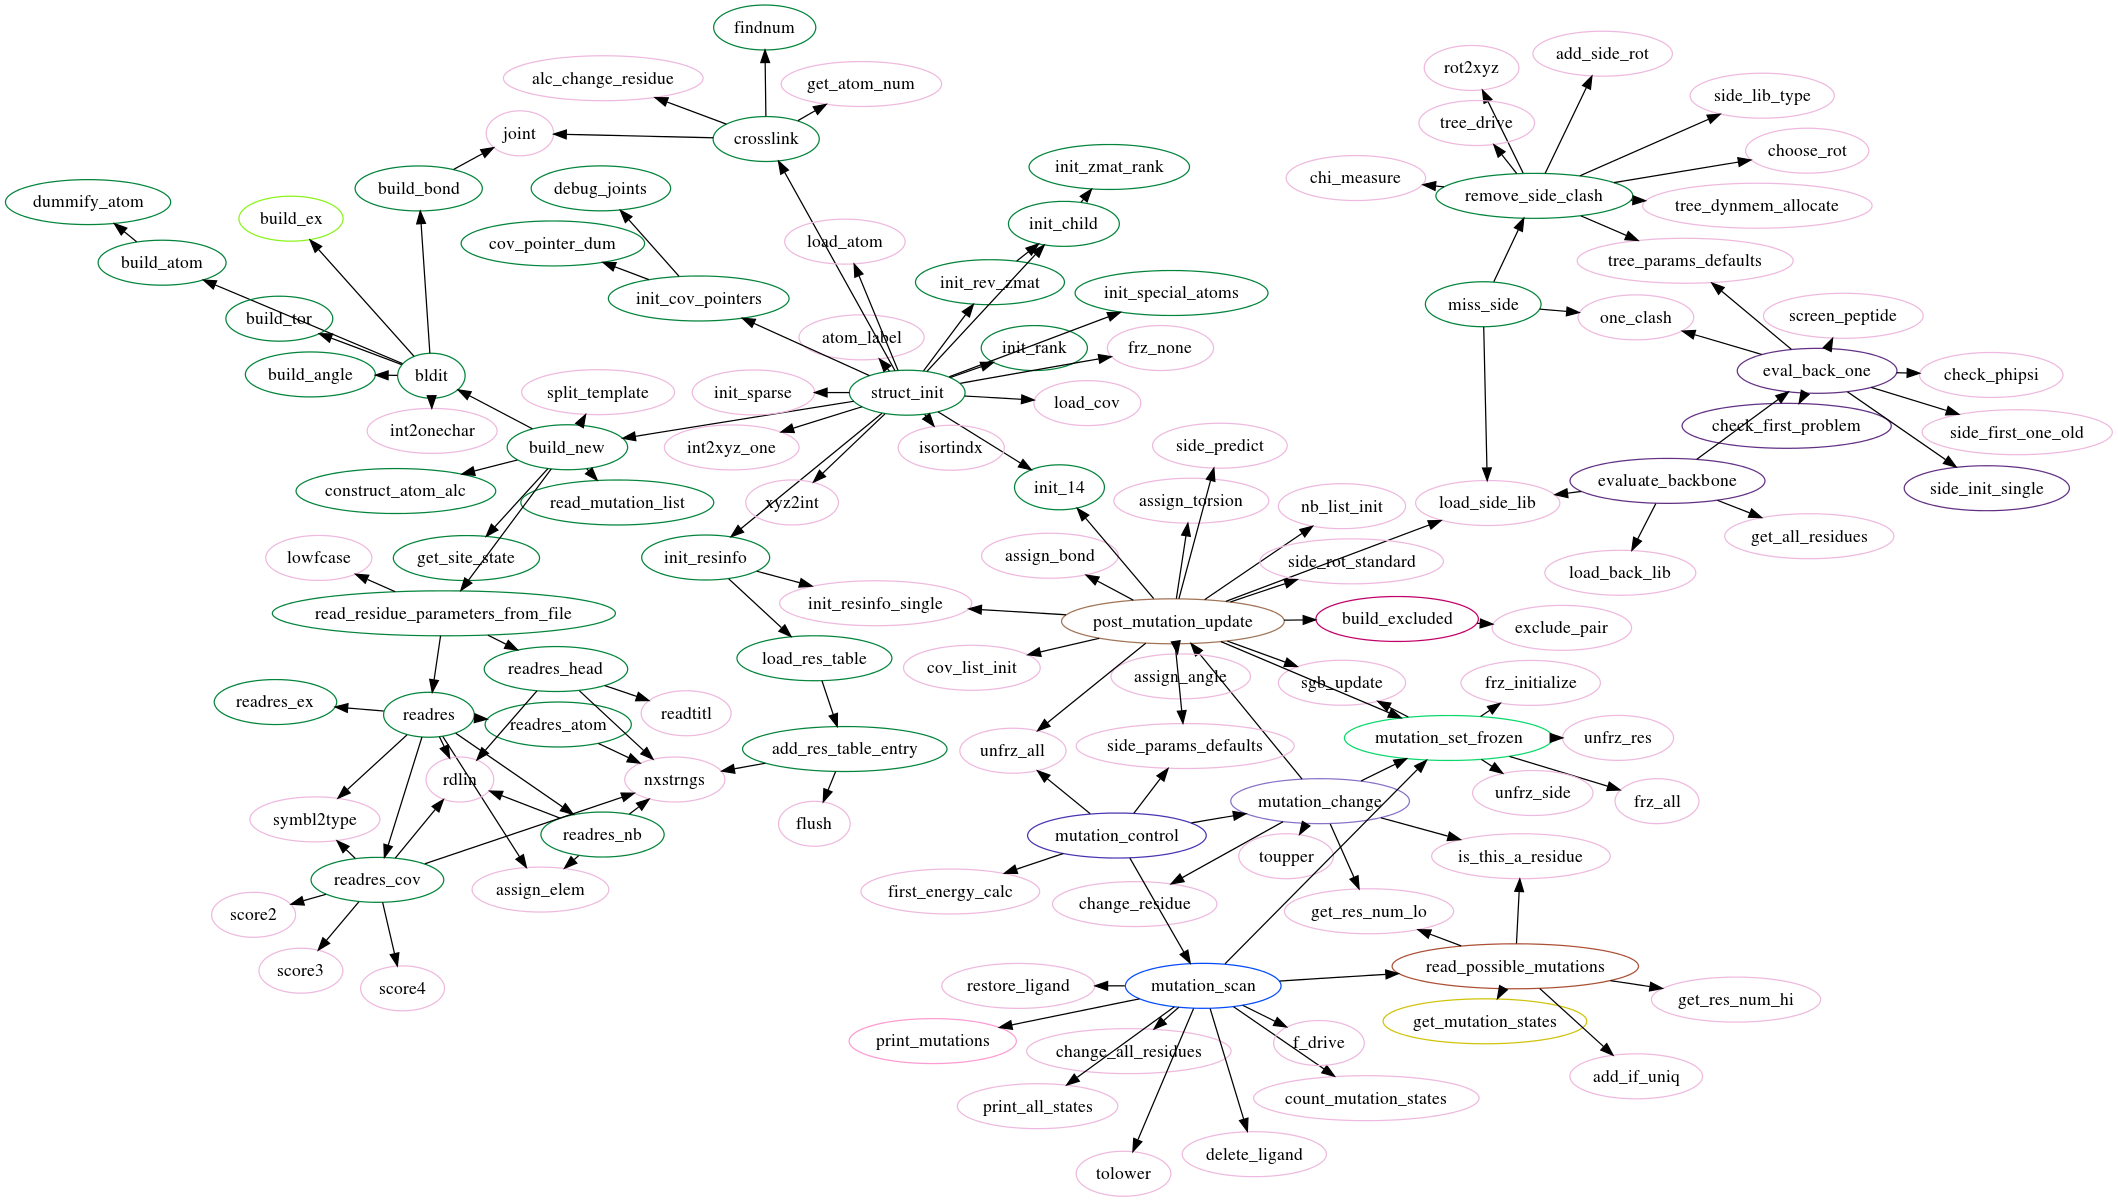
\includegraphics[width=1.0\textwidth,height=0.9\textheight,keepaspectratio]{figures/plop_connected_sfdp.png}
    \caption{An example call graph generated for for the code implementing mutation scanning and certain files having to do with building a structure in memory.
The call graph of the entire program is both too large to display, and too complicated to be useful in development.}
    \label{figure:mutation_call_graph}
\end{figure}

